\documentclass[12pt,dvipdfmx]{jreport}
\usepackage{mthesis}
\usepackage{graphicx,xcolor,amsmath,amssymb,enumitem,url}
\usepackage{bcprules}
\usepackage{listings,lstcoq,lsterlang}

\usepackage{my}

\newtheorem{definition}{定義}
\newtheorem{theorem}{定理}
\newtheorem{lemma}{補題}

\lstdefinestyle{default}{
  language=coq,
  basicstyle={\ttfamily\normalsize},
  breaklines=true,
  % frame=tb,
  framesep=6pt,
  captionpos=b,
  numberstyle=\scriptsize,
  numbers=left,
  numbersep=6pt,
  xleftmargin=12pt,
  aboveskip=1em,
  belowskip=1em,
}
\lstdefinestyle{small}{
  style=default,
  basicstyle={\ttfamily\small},
}
\lstset{
  style=default
}

\年度{平成27年度}
\提出年月{平成28年1月}
\提出年月e{2016. ~Jan}
\題名{定理証明支援系による\\アクターシステムの検証}
\指導教員名{渡部  卓雄}
\職名{准教授}
\研究科{情報理工学}
\専攻{計算工学}
\学籍番号{14M38391}
\氏名{安武  祥平}
\内容梗概{
本研究の目的は,アクターモデルにより構成されたシステムの検証に定理証明支援系が有効であることを明らかにすることである.
アクターモデルは非同期メッセージパッシング方式の並行計算のモデルのひとつであり,
アクターと呼ばれる計算主体が相互にメッセージを送り合うことで計算を進める.
アクターモデルは,アクター同士が共有する状態を持たないことから,各アクターの処理中に何らかのエラーが発生した際には
そのアクターのみを停止や再起動させることによってシステム全体は停止させずに計算を進めるということを行いやすい.
そのためアクターモデルは対障害性が必要なシステムに用いられることが多い.
しかし,そのシステムが確かにある障害に対して耐性があるということを示すのは一般に難しい.

アクターシステムのような並行システムの形式的検証の手法の一つとしてはモデル検査によるアプローチがある。
本研究では、別のアプローチとして定理証明支援系による検証を試みる。
定理証明支援系とは、数学的な命題やプログラムの性質に対して厳密かつ形式的な証明を与えることができるシステムのことである。
本研究では,定理証明支援系によるアクターシステムの検証の有効性を明らかにするために定理証明支援系Coqによるアクターシステムのための検証ライブラリActarioを作成した.
Actarioは,
(1) アクターモデルを使った並行アプリケーションをCoqのDSLを用いて記述できる
(2) アクターモデルの意味論を提供しており,アクターモデル自体の性質を検証できる
(3) 作成したアクターアプリケーションに対してその性質を検証できる
(4) 作成したアクターアプリケーションをErlangのコードに変換できる
という特徴を持っている.
また,Actarioはアクターの名前付けがシステムによって暗黙的に行うことで、ユーザーが一意な名前付けを明示的に行わなくてもよくなっている。
そしてActarioの持つ操作的意味論によって付けられる名前が必ず一意になるということは、形式的に証明されている。
本論文では,簡単な例題を通してActarioの有用性を示す.
}

\begin{document}
\maketitle
\tableofcontents

\chapter{序論}
\label{chapter:intro}

\chapter{背景知識}
\label{chapter:background}

\section{アクターモデル}

アクターモデル\cite{Agha:1986aa}とは、非同期メッセージパッシングに基づいた並行計算のモデルである。
アクターと呼ばれる並行計算の主体が互いにメッセージを送り合うことで計算を進める。
対象となるアクターの名前を指定することでメッセージを送信する。


\subsection{振る舞い}

\emph{振る舞い(behavior)}とは、アクターがメッセージを受け取って何をするか、というものである。
この「何をするか」という部分をアクターの\emph{アクション(action)}と呼ぶ。
アクターのアクションには以下の3つのものがある。

\begin{itemize}
\item 新しいアクターを生成する
\item 他のアクターにメッセージ
\item 自分自身の振る舞いを変える
\end{itemize}


\subsection{配置}

\emph{配置(configuration)}とは、システムの状態のスナップショットのことである。
その時点でのアクターおよびまだ受け取られていないメッセージの集合から構成される。

\subsection{アクターの名前}

アクターがメッセージを送信する際に指定する宛先のことをアクターの\emph{アドレス}またはアクターの\emph{名前}という。これ以降この論文ではアクターの名前で統一する。
アクターモデルではアクターの名前を指定してメッセージを送信するため、アクターの名前が一意であるという性質はアクターモデルの一貫性のために非常に重要なものとなっている。

\subsection{\fairness}

アクターモデルでは\fairness という性質が必ず成り立つ。
\fairness とは、無限にしばしばあるアクターがあるアクションを実行できる状態にあるならば、いつかそのアクションは実行される、というものである。

\fairness が成り立たなければ、例えばあるアクターAとアクターA'が無限に相互通信を行うようなアクターシステムと、あるアクターBとアクターB'が無限に相互通信を行うようなアクターシステムを合成すると、アクターAとアクターA'のみ通信し、アクターBとアクターB'の通信は起きないということが起こりえる。
このような状況を防ぐためにも、\fairness は重要である。


\section{定理証明支援系 Coq}

Coq\cite{Coq}とは、フランス国立情報学自動制御研究所(INRIA)で開発が進められている定理証明支援系と呼ばれるシステムの一つである。
定理証明支援系とは人間が形式的な形で証明を書きやすいように支援するシステムのことである。
Coqでは以下のことが行える。

\begin{itemize}
\item プログラムの仕様の検証や数学的な命題の証明
\item 型理論に基づいた証明の機械的なチェック
\item タクティクと呼ばれる証明の方針を記述していくためのコマンドによる柔軟な証明記述
\item プラグインシステムによる拡張
\item 他の言語へのコード抽出(extraction)
\end{itemize}

例として、ある型\coqi{A}のリストを逆順にする関数\coqi{reverse}を考える。\coqi{reverse}は図\ref{code:background:reverse}のように定義できる。

\begin{figure}
\begin{lstlisting}
Fixpoint reverse (l : list A) :=
  match l with
  | [] => []
  | hd :: tl => reverse tl ++ [hd]
  end.
\end{lstlisting}
\label{code:background:reverse}
\caption{\coqi{reverse}関数の定義}
\end{figure}

リストを逆順にする関数\coqi{reverse}は、二度適用するともとのリストに戻るという性質を持っているので、ここで定義した関数がその声質を満たしているということを確かめるために、証明を行う(証明できなければここで定義した関数は間違った実装になっているということになる)。
Coqでのこの定理の証明は図\ref{code:background:reverse-reverse}のようになる。
ここでは補題\coqi{snoc_reverse}と目的の定理\coqi{reverse_reverse_id}を証明している。
\coqi{Lemma}および\coqi{Theorem}の後ろが命題の名前と命題を表す式になっており、
\coqi{Proof}から\coqi{Qed}までが命題を証明している部分である。証明の部分に書かれているコマンド(\lstinline{intros} や\coqi{induction}などのこと)は証明を進めていく際の方針を表すものであり、これを\emph{タクティク}と呼ぶ。

\begin{figure}
\begin{lstlisting}
Lemma snoc_reverse : forall a l, reverse (l ++ [a]) = a :: reverse l.
Proof.
  intros a l.
  induction l as [ | a' l ].
  - reflexivity.
  - rewrite IHl; reflexivity.
Qed.

Theorem reverse_reverse_id :
  forall l : list A, reverse (reverse l) = l.
Proof.
  intros l.
  induction l as [ | a l ].
  - reflexivity.
  - rewrite snoc_reverse.
    rewrite IHl.
    reflexivity.
Qed.
\end{lstlisting}
\label{code:background:reverse-reverse}
\caption{\coqi{reverse}を二度適用するともとのリストに戻ることの証明}
\end{figure}


\subsection{コード抽出}

CoqにはOCaml, Haskell, Schemeへのコード抽出器がデフォルトで内蔵されている。
抽出器はプラグインの形で実装されており、Coqの型定義・関数定義からMiniMLというMLのサブセットにあたるような言語の抽象構文木に一旦変換され、そこから各言語に変換される。
上の\coqi{reverse}関数をOCamlに向けて変換すると、図\ref{code:background}のようになる。\coqi{Extraction}コマンドでその関数を抽出することができる。
\coqi{Recursive Extraction}コマンドを使うとその関数が依存している型と関数も抽出される。

\begin{figure}
\begin{lstlisting}
Extraction reverse.
(** =>
 * let rec reverse = function
 * | Nil -> Nil
 * | Cons (hd, tl) -> app (reverse tl) (Cons (hd, Nil))
 *)
\end{lstlisting}
\label{code:background:reverse-reverse}
\caption{\coqi{reverse}の抽出}
\end{figure}

%% \subsection{基本的な構文}

%% \begin{figure}
%% \end{figure}
%% これを型コンストラクタと呼ぶ。型を受け取って型を返すような関数とも見れる。
%% これを値コンストラクタと呼ぶ。何か値を受け取って、値コンストラクタの型の値を返すような関数とも見れる。

\section{Erlang}

Erlang\cite{Erlang}は高可用なシステムを作るために作られた動的型付き関数型プログラミング言語である。
並行計算のモデルとしてアクターモデルを採用している。
Erlangにおいて、並行計算の主体はアクターではなくプロセスと呼ばれる。

\subsection{基本的な構文}

本論文で扱うErlangの基本的な構文について説明する。

\begin{description}
\item[変数]\mbox{}\\
  大文字から始まる識別子は変数である。Erlangでは変数は不変であり、再代入することはできない。
\item[アトム]\mbox{}\\
  小文字から始まる識別子は\emph{アトム(atom)}と呼ばれるシンボルである。
\item[組]\mbox{}\\
  波括弧で囲まれ、カンマで句切られた項は組(tuple)である。例えば\lstinline|{Var, atom, 42}|は変数\lstinline{Var}、アトム\lstinline{atom}、数値\lstinline{42}の組である。
\item[関数]\mbox{}\\
  関数は\lstinline[language=Erlang]{$func$($arg1$, $\cdots$, $argn$) -> $expr$.}という形で定義する。
  同じ関数名で、異なった数の引数をとるような関数も定義でき、関数を呼び出す側は関数名の後ろにスラッシュと数を書くと、その数の引数をとる関数と指定できる。
  これを関数のアリティという。
\item[パターンマッチ]\mbox{}\\
  \lstinline[language=Erlang]{case $expr$ of $pat1$ -> $expr1$; $\cdots$; $patn$ -> $exprn$ end.}という構文で式のパターンマッチを行うことができる。
\end{description}

\subsection{並行計算のための関数と構文}

Erlang並行計算の基本的な関数および構文について解説する。

\begin{description}
\item<\lstinline{spawn/1}>\mbox{}\\
  \lstinline{spawn/1}は新しいプロセスを作る関数である。新しいプロセスで行う処理が書かれた関数を受け取り、プロセスのIDを返す。\lstinline{spawn}関数はアリティが1から4までのものが定義されているが、本論文ではアリティが1のものだけを扱う。
\item<\lstinline{self/0}>\mbox{}\\
  \lstinline{self/0}は関数であり、この関数を呼び出したプロセスのIDを返す。
\item<\lstinline{!}>\mbox{}\\
  \lstinline{!}は二項演算子であり、左手で指定したプロセスIDを持つプロセスに向けて、右手で指定した値を送信するという構文である。
\item<\lstinline{receive}>\mbox{}\\
  \lstinline{receive}はそのプロセスに向けて送られたメッセージを受け取り、パターンマッチを行う構文である。
\end{description}

\chapter{検証フレームワーク Actario}
\label{chapter:overview}

本章では、本研究で作成したアクターシステムの検証フレームワーク Actario についての概要を説明する。
Actario では、

\section{概要}

図 \ref{img:overview:workflow} は、Actario を用いてアクターシステムを検証する際のワークフローである。
まず Actario が提供するアクターシステムを記述するための記法を使って、検証したいアクターシステムを記述する。
次にそのアクターシステムが満たしているべき仕様を記述し、それを Actario が提供する証明の機構によって証明する。
最後に Actario が持つ Erlang へのコード抽出機を用いて実装を Erlang に抽出する。

\begin{figure}[tp]
  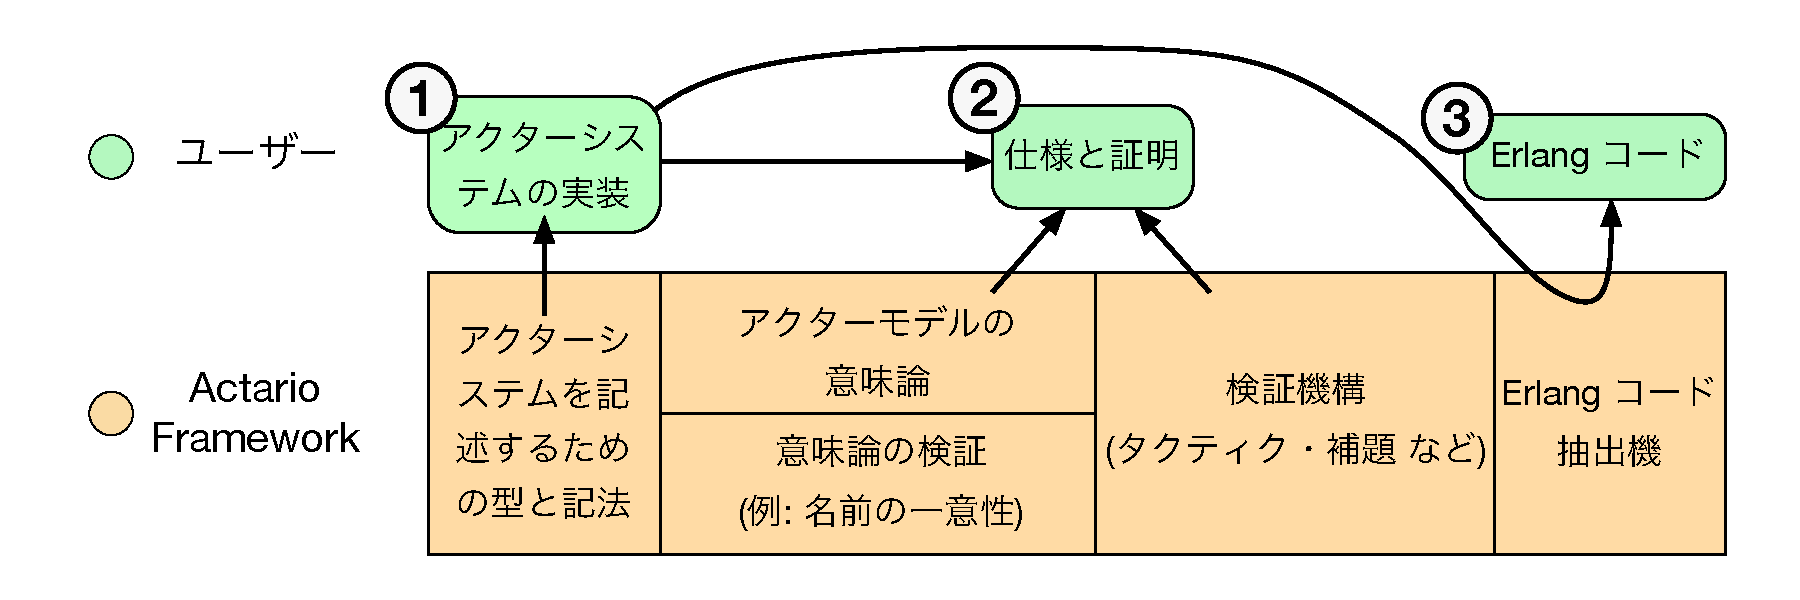
\includegraphics[width=14cm]{./img/overview/workflow.pdf}
  \label{img:overview:workflow}
  \caption{Actario のワークフロー}
\end{figure}

\section{例: 階乗計算アクターシステム}

このアクターシステムは、一つのアクターのなかで階乗を計算するのではなく、
次に何の数を掛けるかという継続を持っているアクターを生成しながら、
階乗を計算する。(?)
図 \ref{img:overview:fact} はこのアクターシステムに $3$ を与えたときの動きを表した図である。

\begin{figure}[tp]
  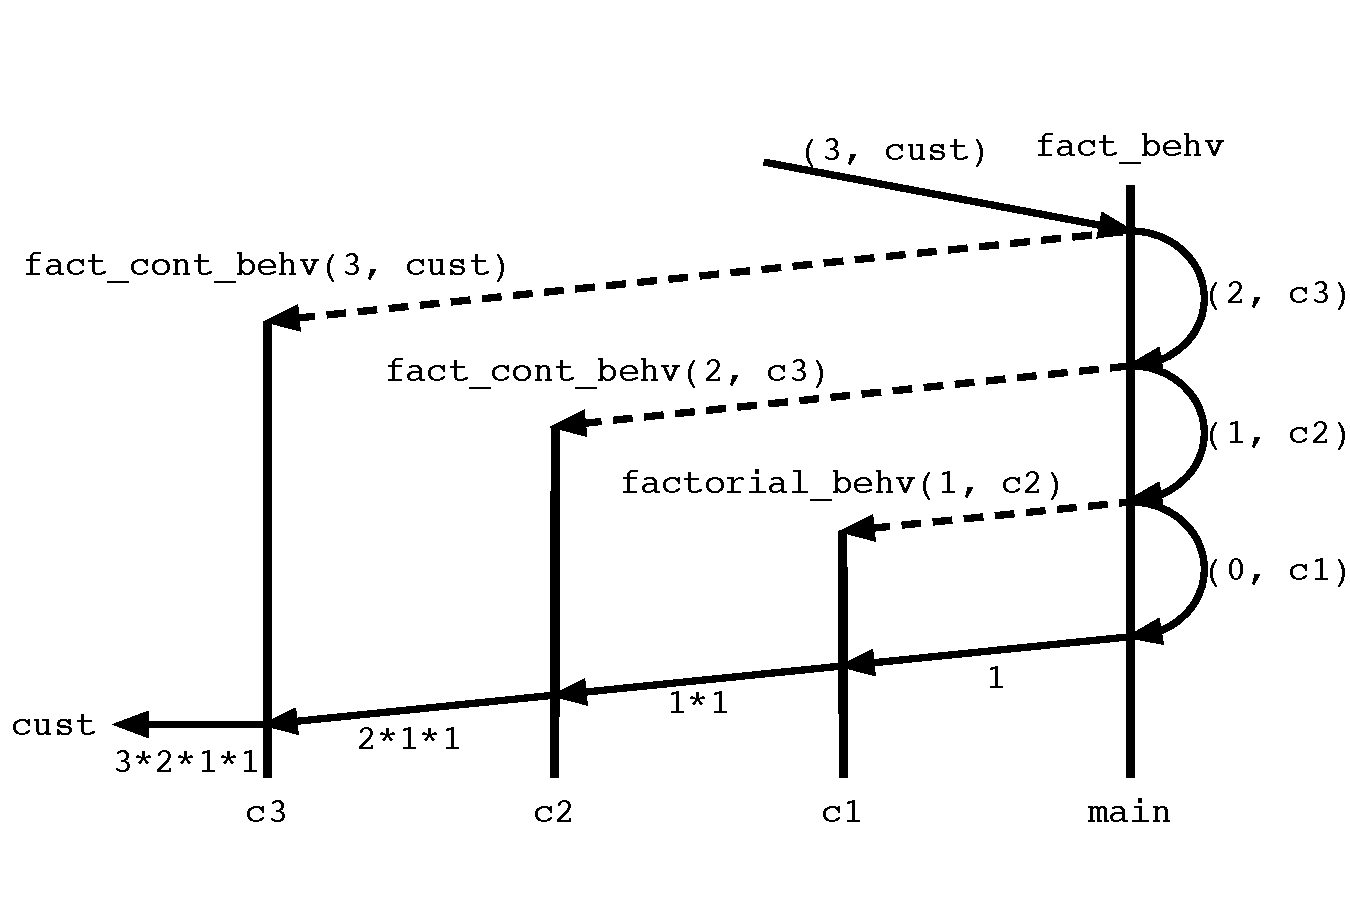
\includegraphics[width=14cm]{./img/overview/fact.pdf}
  \label{img:overview:fact}
  \caption{fact 3}
\end{figure}

Actario を用いると、階乗計算アクターシステムは図 \ref{code:overview:fact-impl} のように記述することができる。

\begin{figure}[tp]
  \lstinputlisting{./code/overview/fact_impl.v}
  \label{code:overview:fact-impl}
  \caption{階乗計算アクターシステム}
\end{figure}

また、証明の例として、「このアクターシステムは階乗を計算する」ということを証明する。
階乗を計算するということはつまりメッセージとして送られた任意の自然数 $n$ に対して、$n!$ を返信するということなので、
命題は図 \ref{code:overview:fact-spec} のように記述することができる。

\begin{figure}[tp]
  \begin{lstlisting}
    dummy
  \end{lstlisting}
  \label{code:overview:fact-spec}
  \caption{命題の定義}
\end{figure}

そして、この命題は図 \ref{code:overview:fact-proof} のように証明することができる。
証明の方針としては、$n$ に対しての帰納法で証明する。

\begin{figure}[tp]
  \begin{lstlisting}
    dummy
  \end{lstlisting}
  \label{code:overview:fact-proof}
  \caption{証明}
\end{figure}

\chapter{アクターモデルの形式化}
\label{chapter:formalization}

本章では、Actarioにおいてアクターモデルをどのように形式化を行っているかということを説明する。
まず、意味論の形式化、名前付け、
障害と回復、fairnessの形式化

\section{意味論の形式化}

まずアクターモデルの操作的意味論の形式化をCoqで行う。

アクターの名前

配置(configuration)は

アクターモデルの操作的意味をconfigurationのラベル付き遷移システムとして定式化する。
これ以降用いる記号を図~\ref{expr:formalization:config}のように定義する。

\begin{figure}[t]
  \begin{displaymath}
    \begin{array}{rclcl}
      c & \in & \textit{Configuration} & =   & \textit{Set(InFlight)} \times \textit{Set(Actor)} \\
      a & \in & \textit{Actor}  & =   & \textit{Name} \times \textit{Actions} \times \mathbb{N} \\
      n & \in & \textit{Name}   & ::= & \textsf{toplevel}(s) \\
        &     &                 &   | & \textsf{generated}(g, n) \\
      m & \in & \textit{Message} & =  & \textit{Name} + \textit{PrimVal} + \\
        &     &                 &     & \textit{Message} \times \cdots \times \textit{Message} \\
      i & \in & \textit{InFlight} & = & \textit{Name} \times \textit{Name} \times \textit{Message} \\
      b & \in & \textit{Behavior} & = & \textit{Message} \rightarrow \textit{Actions} \\
      \alpha & \in & \textit{Actions} & ::= & \textsf{send}(n, m, \alpha) \\
        &     &                 &   | & \textsf{new}(b, \kappa) \\
        &     &                 &   | & \textsf{self}(\kappa) \\
        &     &                 &   | & \textsf{become}(b) \\
      l & \in & \textit{Label}  & ::= & \textsf{Receive}(n, n, m) \\
        &     &                 &   | & \textsf{Send}(n, n, m) \\
        &     &                 &   | & \textsf{New}(n) \\
        &     &                 &   | & \textsf{Self}(n) \\
      \kappa & \in & \textit{Name} \rightarrow \textit{Actions} \\
      g & \in & \mathbb{N} & &
    \end{array}
  \end{displaymath}
  \caption{Configuration}\label{expr:formalization:config}
\end{figure}


\begin{figure}[t]
  \begin{displaymath}
    \begin{array}{rcl}
      (I \uplus \{(n_{\textrm{to}}, n_{\textrm{from}}, m)\}, A \cup \{(n_{\textrm{to}}, \textsf{become}(b), g)\}) &
      \overset{\textsf{Receive}(n_{\textrm{to}}, n_{\textrm{from}}, m)}{\leadsto} &
      (I, A \cup \{(n_{\textrm{to}}, b(m), g)\})
      \hfill \textsc{(Receive)} \\[1ex]

      (I, A \cup \{(n_{\textrm{from}}, \textsf{send}(n_{\textrm{to}}, m, \alpha), g)\}) &
      \overset{\textsf{Send}(n_{\textrm{from}}, n_{\textrm{to}}, m)}{\leadsto} &
      (I \uplus \{(n_{\textrm{to}}, n_{\textrm{from}}, m)\}, A \cup \{(n_{\textrm{from}}, \alpha, g)\}) \\
      & & \hfill \textsc{(Send)} \\[1ex]

      (I, A \cup \{(n, \textsf{new}(b, \kappa), g)\}) &
      \overset{\textsf{New}(n')}{\leadsto} &
      (I, A \cup \{(n, \kappa(n'), g + 1), (n', \textsf{become}(b), 0)\}) \\
      & & \hfill \textrm{where}\ n' := \textsf{generated}(g, n) \\
      & & \hfill \textsc{(New)} \\[1ex]

      (I, A \cup \{(n, \textsf{self}(\kappa), g)\}) &
      \overset{\textsf{Self}(n)}{\leadsto} &
      (I, A \cup \{n, \kappa(n), g\})
      \hfill \textsc{(Self)}
    \end{array}
  \end{displaymath}
  \caption{labeled transition semantics}\label{expr:formalization:semantics}
\end{figure}



\subsection{名前の一意性の証明}

この名前付けの方法によって生成された名前は必ず一意になるということを証明する。
これを証明するために、名前に関する\textit{trans invariant}という遷移の間で変わらない性質を定義する。
trans invariant は以下のように3つの述語\texttt{chain}, \texttt{gen\_fresh}, \texttt{no\_dup}の組で定義される。

\begin{displaymath}
  \begin{array}{l}
    \texttt{trans\_invariant}(c) := \\
    \quad \texttt{chain}(c) \wedge \texttt{gen\_fresh}(c) \wedge \texttt{no\_dup}(c)
  \end{array}
\end{displaymath}

\texttt{chain}, \texttt{gen\_fresh}, \texttt{no\_dup}の簡単な説明は以下のとおりである。

\begin{description}[style=nextline,leftmargin=12pt,parsep=0pt]
\item[\texttt{chain}]
  配置の各アクターについて、そのアクターが他のアクターから生成されたものであるなら親アクターはその配置に存在している。
\item[\texttt{gen\_fresh}]
  配置の各アクターについて、そのアクターが次に生成するアクターの名前は配置内で新しい名前である。
\item[\texttt{no\_dup}]
  配置のすべてのアクターの名前は一意である。
\end{description}

\subsubsection{Functions}

Before starting the explanation and the proof, we define some functions used in this section.

\begin{description}[style=nextline,leftmargin=12pt,parsep=0pt]
\item[\texttt{actors} $: \textit{Configuration} \rightarrow \textit{Set(Actor)}$]
  \texttt{actors} returns the set of actors in the given configuration.
\item[\texttt{parent} $: \textit{Actor} \rightarrow \textit{Actor}$]
  \texttt{parent} returns the parent actor of the given actor.
  If the given actor is toplevel actor, the function returns nothing. % null?
\item[\texttt{gen\_number} $: \textit{Actor} \rightarrow \mathbb{N}$]
  \texttt{gen\_number} returns generated number of the name of the given actor.
  If the given actor is toplevel actor, the function returns nothing.
\item[\texttt{next\_number} $: \textit{Actor} \rightarrow \mathbb{N}$]
  \texttt{next\_number} returns next generation number of the given actor.
\item[\texttt{name} $: \textit{Actor} \rightarrow \textit{Name}$]
  \texttt{name} returns the name of the given actor.
\item[\texttt{names} $: \textit{Set(Actor)} \rightarrow \textit{Set(Name)}$]
  \texttt{names} returns names of the given set of actors.
\end{description}

\subsubsection{Chain Property}
We define a predicate of configuration, called \texttt{chain}.
\texttt{chain} is the predicate that, for each actor in the given configuration, if it is generated by another actor, the parent actor is also in the configuration.
\texttt{chain} is defined as the following.

\begin{displaymath}
  \begin{array}{l}
    \texttt{chain}(c) := \\
    \quad \forall a \in \texttt{actors}(c), \forall p, p = \texttt{parent}(a) \Rightarrow p \in \texttt{actors}(c)
  \end{array}
\end{displaymath}

Then, we can prove \textit{chain preservation property} that chain is preserved between any transitions.
The proof is by case analysis on the label.
\texttt{chain} is decided by only actor names, and the transition which have a possibility to change the names in the configuration is only \textsc{New} transition.
Therefore, we consider only the case of \textsc{New} transition.

\begin{lemma}{chain preservation}
\begin{displaymath}
  \begin{array}{l}
    \forall c, c' \in \textit{Configuration}, \forall l \in \textit{Label}, \\
    \quad \texttt{chain}(c) \wedge c \overset{l}{\leadsto} c' \Rightarrow \texttt{chain}(c')
  \end{array}
\end{displaymath}
\end{lemma}

\subsubsection{Gen Fresh Property}
We define \texttt{gen\_fresh} predicate that, for each actor in the configuration, the name of its child is always fresh.
The definition of \texttt{gen\_fresh} is complicated a little.
We translate the proposition that next generated name is fresh to the following.

\begin{displaymath}
  \begin{array}{l}
    \texttt{gen\_fresh}(c) := \\
    \quad \forall a \in \texttt{actors}(c), \forall p \in \texttt{actors}(c), p = \texttt{parent}(a) \Rightarrow \\
    \quad \quad \quad \texttt{gen\_number}(a) < \texttt{next\_number}(p)
  \end{array}
\end{displaymath}


It is guaranteed that the actor name generated in the next is fresh if satisfying \texttt{gen\_fresh} predicate by the relation of next generation numbers and actor names. %% For each actor in the configuration, if its parent is in the configuration, the next generation number of the parent actor is greater than the generation number of the name of the child actor.
However, the actor name generated after the next is not always fresh name.
For example, if there are two actors ($A$ and $B$) that have the same name and the same next generation number and actor $A$ generates a child actor and actor $B$ generates a child actor, although \texttt{gen\_fresh} holds, these child actors have the same name.
Furthermore, if the parent of the actor $A$ does not exist in the configuration and the parent of the parent exists in the configuration, and the parent of the parent actor generates an actor and it also generates an actor, then the name is possible to have the same as $A$'s one.

%% つまり、あるアクターについて、システム内に親アクターがいる場合、親アクターが次に生成する番号は自分の番号よりも大きい、ということにより、次に生成するアクターの名前が被らないようになっている。
%% ただし、次に生成するアクターの名前は fresh でもその次に生成するアクターは fresh ではないこともある。
%% 例えば、同じ名前でかつ次の generation number も同じという2つのアクターがいた場合、まず片方のアクターが生成するアクターの名前は fresh だが、その次にもう片方のアクターがアクターを生成したとすると、名前が被ってしまう。
%% また、親アクターがシステム内に存在せずに、親の親は存在しているという場合、親の親が次に生成するアクターの名前は被らないが、その子アクターが次に生成する名前は被ってしまう可能性がある。(図?)

Thus, to prove \textit{gen fresh preservation} proposition that \texttt{gen\_fresh} is preserved between transitions, it is necessary to use \texttt{chain} and \texttt{no\_dup} as hypotheses.
%% The proof is by ...
%% 以上のように gen\_fresh だけでは gen\_fresh を導けないので、gen\_fresh の証明には chain と no\_dup の性質が必要になる。

\begin{lemma}{gen fresh preservation}
\begin{displaymath}
  \begin{array}{l}
    \forall c, c' \in \textit{Configuration}, \forall l \in \textit{Label}, \\
    \quad \texttt{chain}(c) \wedge \texttt{gen\_fresh}(c) \wedge \texttt{no\_dup}(c) \wedge c \overset{l}{\leadsto} c' \Rightarrow \\
    \quad \texttt{gen\_fresh}(c')
  \end{array}
\end{displaymath}
\end{lemma}

\subsubsection{No Dup Property}
We define \texttt{no\_dup} predicate that all actor names in the given configuration are unique.
This is the property we have to prove.
\texttt{no\_dup} is defined as the following.

\begin{displaymath}
  \begin{array}{l}
    \texttt{no\_dup}(c) := \\
    \quad \forall a \in \texttt{actors}(c), \texttt{name}(a) \notin
    \texttt{names}(\texttt{actors}(c) \setminus \{a\})
  \end{array}
\end{displaymath}

We proved \textit{no dup preservation} property defined as the following.
It represents that if the actor names in the configuration is not duplicate and the next generated actor name is fresh, then \texttt{no\_dup} holds in the next configuration.

\begin{lemma}{no dup preservation}
\begin{displaymath}
  \begin{array}{l}
    \forall c, c' \in \textit{Configuration}, \forall l \in \textit{Label}, \\
    \quad \texttt{gen\_fresh}(c) \wedge \texttt{no\_dup}(c) \wedge c \overset{l}{\leadsto} c' \Rightarrow \texttt{no\_dup}(c')
  \end{array}
\end{displaymath}
\end{lemma}

\subsubsection{Proof of Name Uniqueness Property}
Then, we start to prove name uniqueness.
First, we prove trans invariant preservation that trans invariant is preserved between transitions.
This is obvious by chain preservation, gen fresh preservation and no dup preservation.
\begin{lemma}{trans invariant preservation}
  \begin{displaymath}
    \begin{array}{l}
      \forall c, c' \in \textit{Configuration}, \forall l \in \textit{Label}, \\
      \quad \texttt{trans\_invariant}(c) \wedge c \overset{l}{\leadsto} c' \Rightarrow \\
      \quad \texttt{trans\_invariant}(c')
    \end{array}
  \end{displaymath}
\end{lemma}

Next, we prove that if trans invariant holds in initial configuration, trans invariant holds after arbitrary transitions.

%% 次に初期状態について trans\_invariant が成り立っていれば、任意回の遷移後も trans\_invariant が成り立つということをを証明する。

\begin{lemma}{trans invariant preservation star}
  \begin{displaymath}
    \begin{array}{l}
      \forall c, c' \in \textit{Configuration}, \forall l \in \textit{Label}, \\
      \quad \texttt{trans\_invariant}(c) \wedge c \overset{l}{\leadsto\star} c' \Rightarrow \\
      \quad \texttt{trans\_invariant}(c')
    \end{array}
  \end{displaymath}
\end{lemma}
$c \overset{l}{\leadsto\star} c'$ represents reflexive transitive closure of transition.
The proof is by induction of reflexive transitive closure of transition and trans invariant preservation.

Finally, we can prove name uniqueness.
\begin{theorem}{name uniqueness}
  \begin{displaymath}
    \begin{array}{l}
      \forall c, c' \in \textit{Configuration}, \forall l \in \textit{Label}, \\
      \quad \texttt{trans\_invariant}(c) \wedge c \overset{l}{\leadsto\star} c' \Rightarrow \texttt{no\_dup}(c')
    \end{array}
  \end{displaymath}
\end{theorem}
This is obvious by trans invariant preservation star because \texttt{no\_dup} is in \texttt{trans\_invariant}.


\section{障害と回復の形式化}

\section{Fairnessの形式化}

Fairnessとは、アクターモデルが持つ性質で、発火する(?)可能性があるものはいつか発火されるというものである。
通常、Fairnessを表現する際には時相論理が必要になるが、Coqは時相論理はサポートしていない。
そのため、配置の遷移列である遷移パスを使ってFairnessを表現する。
この手法はAppl$\pi$\cite{}で用いられている手法である。Appl$\pi$は$\pi$計算のためのライブラリであるが、Fairnessの定義方法についてはアクターモデルに対しても同様に用いることができる。

\subsection{遷移パス}
遷移パスは自然数$\mathbb{N}$から\texttt{option config}型への関数として定義する (図~\ref{code:formalization:path})。
定義域の自然数は、初期状態から何回目の遷移によってこの配置になったかという番号である。この番号をインデックスと呼ぶ。
値域はそのインデックスに対応する配置を表す。\texttt{config}型ではなく\texttt{option config}型になっているのは、これ以上遷移ができないパスも表したいからである。つまり、これ以上遷移ができない配置のインデックスを$n$とすると、$\forall m > 0, n + m$に遷移パス関数を適用した結果は\texttt{None}になる。

\begin{figure}[tp]
  \begin{lstlisting}
    Definition path := nat -> option config.
  \end{lstlisting}
  \label{code:formalization:path}
  \caption{遷移パスの定義}
\end{figure}

また、与えられた遷移パスが確かに遷移パスとしての仕様を満たしているか、という述語を定義する(図~\ref{code:formalization:path-spec})。
すべてのインデックス$i$について、$i$番目の配置が存在するならば、$i+1$番目の配置が存在するならそれは遷移できるものか、それ以上遷移できない。$i$番目の配置が存在しないならば、その次の配置も存在しない、という意味である。

\begin{figure}[tp]
  \begin{lstlisting}
Definition is_transition_path (p : path) : Prop :=
  forall n,
    (forall c, p n = Some c ->
      (exists c' l, p (S n) = Some c' /\
        c ~(l)~> c') \/
      p (S n) = None) /\
    (p n = None -> p (S n) = None).
  \end{lstlisting}
  \label{code:formalization:path-spec}
  \caption{遷移パスの仕様}
\end{figure}

\subsection{遷移可能性}
次に、与えられた配置が与えられたラベルでもって遷移ができるという述語を定義する。これを遷移可能性(enabled)と呼ぶ。
Actarioでは、遷移可能性はある配置からあるラベルによって遷移した先の配置が存在すると定義する (図~\ref{code:formalization:enabled})。

\begin{figure}[tp]
  \begin{lstlisting}
Definition enabled (c : config) (l : label) : Prop := exists c', c ~(l)~> c'.
  \end{lstlisting}
  \label{code:formalization:enabled}
  \caption{遷移可能性}
\end{figure}

\subsection{Infinitely Often Enabled}
無限にしばしば遷移可能になる
We define the predicate that the transition is infinitely often enabled in the transition path.
It is named \texttt{infinitely often enabled}.
%% これは、すべての index n について、n 番目の configuration があるラベルによって遷移が可能ならば、その先そのラベルによって遷移が可能になる configuration が存在する、と定義する。

\begin{lstlisting}
Definition infinitely_often_enabled
    (l : label) (p : path) : Prop :=
  forall n c, p n = Some c ->
    enabled c l ->
    exists m c', m > n /\
      p m = Some c' /\
      enabled c' l.
\end{lstlisting}


\subsection{Eventually Processed}
We define \texttt{eventually processed} that is the predicate of label and transition path.
It represents that the transition with the label is processed eventually in the path.
It is defined as follows.

\begin{lstlisting}
Definition eventually_processed
    (l : label) (p : path) : Prop :=
  exists n c c',
    p n = Some c /\
    p (S n) = Some c' /\
    c ~(l)~> c'.
\end{lstlisting}


\subsection{Definition of Fairness}
Then we can define \texttt{fairness} predicate for transition path.
For the given transition path and for each label, if \texttt{infinitely often enabled} holds, then \texttt{eventually processed} holds.
\texttt{is postfix of} predicate is used for representing 'infinite'.
If \texttt{is postfix of} is not used, the transition may not be processed after the transition is processed although the transition is processed in whole the path.
To prevent it, if \texttt{inifinitely often enabled} holds then \texttt{eventually processed} holds for arbitrary postfix path by using \texttt{is postfix path}.

\begin{lstlisting}
Definition is_postfix_of
    (p' p : path) : Prop :=
  exists n, (forall m, p' m = p (m + n)).

Definition fairness : Prop :=
  forall p p', is_postfix_of p' p ->
    (forall l,
      infinitely_often_enabled l p' ->
      eventually_processed l p').
\end{lstlisting}

\chapter{証明機構}
\label{chapter:proof}

本章では,Actarioでのアクターシステムに関する命題の定義方法およびその証明の機構について説明する.
まず遷移パスを使って行う\fairness の形式化について説明する.
次に\fairness の形式化を行う際に用いた,この先いつかある事柄が成り立つ,というような述語を使って,初期状態からいつか必ずあるラベルで遷移するというような性質を表す述語を定義する.
その後,証明を行う際に用いる遷移可能なラベルと遷移後の配置を計算するための関数について説明し,
最後に遷移パスを使って証明を行う方法について説明する.

\section{\fairness の形式化}
\fairness とは,アクターモデルが持つ性質で,無限にしばしばあるラベルで遷移しうるならば必ずいつかそのラベルで遷移するというものである.
アクターモデルでは必ず\fairness が成り立っており,これを前提としなければ証明できない性質もあるため,まず\fairness の形式化を行う.
また,\fairness を形式化する際に使う,この先いつかある事柄が成り立つ,というような述語はActarioの証明機構でも使っているので,その説明も行う.

通常,\fairness を表現する際には時相論理が必要になるが,Coqは時相論理はサポートしていない.
そのため,配置の遷移列である遷移パスを使って\fairness を表現する.
この手法はAffeldtらによるAppl$\pi$\cite{Affeldt200817}で用いられている手法である.Appl$\pi$は$\pi$計算のためのライブラリであるが,\fairness の定義方法についてはアクターモデルに対しても同様に用いることができる.

\subsection{遷移パス}
遷移パスは自然数$\mathbb{N}$から\texttt{option config}型への関数として定義する (図~\ref{code:formalization:path}).\texttt{config}型は配置を表す型であり,\texttt{option}は型引数で受け取った型の値を持つか,または値がないことを表す型(型コンストラクタ)である.
定義域の自然数は,初期状態から何回目の遷移によってこの配置になったかという番号である.この番号をインデックスと呼ぶ.
値域はそのインデックスに対応する配置を表す.\texttt{config}型ではなく\texttt{option config}型になっているのは,これ以上遷移ができないパスも表したいからである.つまり,これ以上遷移ができない配置のインデックスを$n$とすると,$\forall m > 0, n + m$に遷移パス関数を適用した結果は\texttt{None}になる.

\begin{figure}[tp]
\begin{lstlisting}
Definition path := nat -> option config.
\end{lstlisting}
  \caption{遷移パスの定義}\label{code:formalization:path}
\end{figure}

また,遷移パスの仕様を,パスに対する述語の形で定義する(図\ref{code:formalization:path-spec}).
すべてのインデックス$i$について,$i$番目の配置が存在するならば,$i+1$番目の配置が存在するならそれは遷移できるものか,それ以上遷移できない.$i$番目の配置が存在しないならば,その次の配置も存在しない,という意味である.

\begin{figure}[tp]
\begin{lstlisting}
Definition is_transition_path (p : path) : Prop :=
  forall i,
    (forall c, p i = Some c ->
       ((forall c' l, ~ (c ~(l)~> c')) -> p (S i) = None) \/
       (exists c', p (S i) = Some c' -> exists l, c ~(l)~> c')) /\
    (p i = None -> p (S i) = None).
\end{lstlisting}
  \caption{遷移パスの仕様}\label{code:formalization:path-spec}
\end{figure}

配置はアクターの集合であるため,本来はその中でアクターの順序はない.しかし,Actarioでの定義はアクターのリストになっており,順序がある.
ラベル付き遷移システムの各遷移の定義(付録\ref{appendix:trans})では入れ替えて等しいものとしているため,遷移パスの各配置も順序を入れ替えられるようにしてよい.
この命題は以下のようになるが,遷移パスは実際には関数であるためこの命題は証明できない(関数の返り値は引数に応じて一意に決まるため).
よってこれは公理とする(図\ref{code:proof:path-perm}).また,ここでの$permutation$は,2つのリストに対してその要素の順序を入れ替えると等しくなるということを表す述語である.

\begin{displaymath}
  \begin{array}{l}
    \forall c, c' \in \textit{Configuration}, permutation(c, c') \rightarrow \\
    \quad \forall p \in \textit{Path}, \forall i \in \mathbb{N}, \\
    \quad \quad \quad p(i) = c \rightarrow p(i) = c'
  \end{array}
\end{displaymath}

\begin{figure}[tp]
\begin{lstlisting}
Axiom path_perm :
  forall p i c c',
    is_transition_path p ->
    Permutation c c' ->
    p i = Some c ->
    p i = Some c'.
\end{lstlisting}
  \caption{遷移パスの配置の入れ替え}\label{code:proof:path-perm}
\end{figure}

\subsection{\enabled}
次に,与えられた配置が与えられたラベルでもって遷移ができるという述語を定義する.これを\emph{\enabled (enabled)}と呼ぶ.
Actarioでは,\enabled はある配置からあるラベルによって遷移した先の配置が存在すると定義する (図\ref{code:formalization:enabled}).

\begin{figure}[tp]
\begin{lstlisting}
Definition enabled (c : config) (l : label) : Prop :=
  exists c', c ~(l)~> c'.
\end{lstlisting}
  \caption{\enabled}\label{code:formalization:enabled}
\end{figure}

\subsection{Inifinitely Often Enabled}
次に,無限にしばしば\enabled になるという述語infinitely often enabledを定義する(図\ref{code:proof:infinitely-often-enabled}).
これは,すべてのインデックス$i$について,$i$番目の配置があるラベルによって遷移可能であるならば,その先そのラベルによって遷移が可能になる配置が存在する,という意味である.

\begin{figure}
\begin{lstlisting}
Definition infinitely_often_enabled (l : label)
                                    (p : path) : Prop :=
  forall i c, p i = Some c ->
    enabled c l ->
    exists i' c',
      i < i' /\
      p i' = Some c' /\
      enabled c' l.
\end{lstlisting}
\caption{infinitely often enabled}\label{code:proof:infinitely-often-enabled}
\end{figure}

\subsection{Eventually Processed}
次に,いつかあるラベルによって遷移が起きるという述語eventually processedを定義する(図\ref{code:proof:eventually-processed}).
これはこの遷移パス内でラベル$l$による遷移が存在するという意味である.

\begin{figure}
\begin{lstlisting}
Definition eventually_processed (l : label) (p : path) : Prop :=
  exists n c c',
    p n = Some c /\ p (S n) = Some c' /\ c ~(l)~> c'.
\end{lstlisting}
\caption{eventually processed}\label{code:proof:eventually-processed}
\end{figure}


\subsection{Fairness}
以上を使って,\fairness は図\ref{code:formalization:fairness}のように定義できる.
任意の遷移パスと任意のラベルにおいて,もし無限にしばしばそのラベルで遷移可能になるならば,いつかはそのラベルでの遷移が起きるという意味である.
なお,\coqi{is_postfix_of}という述語は,あるパスがあるパスのはじめの$n$回の遷移を除いたものであり,\fairness の定義においてはこれから先常にこれが成り立つことを表すために使われている.
もし\coqi{is_postfix_of}がなければ,そのパス全体ではあるラベルで遷移が起こることは保証されるが,遷移が起こったあとは無限にしばしば遷移可能になっても遷移しないようなパスも許される.
これを防ぐために,\coqi{is_postfix_of}を用いて,実際に遷移が起きてもその先無限にしばしば遷移可能になることがあればその部分でもいつかは遷移が起きるということを強制している.

\begin{figure}
\begin{lstlisting}
Definition is_postfix_of (p' p : path) : Prop :=
  exists n, (forall m, p' m = p (m + n)).

Definition fairness : Prop :=
  forall p p', is_postfix_of p' p ->
    (forall l,
      infinitely_often_enabled l p' ->
      eventually_processed l p').
\end{lstlisting}
\caption{\fairness の定義}\label{code:formalization:fairness}
\end{figure}

\section{命題の定義}

本節では,アクターモデルによるシステムの性質を記述するための述語について説明する.
アクターシステムの性質を表す際に便利な述語を,前節で定義した\coqi{eventually_processed}を使って定義する.
アクターモデルによって構成されたシステムは,何回遷移が起きるかわからないがいつかはこの状態になってほしい,もしくはこのアクションが実行される,というような性質を検証したいことが多い.
よって図\ref{code:proof:ev-do-label}のように,初期状態とラベルの述語とする.

\begin{figure}
\begin{lstlisting}
Definition eventually_do_label (c0 : config) (l : label) :=
  forall p : path,
    p 0 = Some c0 ->
    is_transition_path p ->
    eventually_processed l p.
\end{lstlisting}
\caption{性質に関する述語の定義}\label{code:proof:ev-do-label}
\end{figure}

\section{遷移可能なラベルと遷移後の配置の計算}

Actarioにおけるアクターシステムの性質の証明の方針は,初期状態から考えられる遷移を一つずつ追っていくというものである.
しかし,素朴に一つずつの遷移を追うと,ユーザーが遷移毎に遷移前の配置から遷移後の配置を予想して書き出す必要が出てしまう.
こうすると証明が非常に煩雑になってしまうため,配置から遷移可能なラベルの集合,配置から各ラベルによって遷移した後の配置は決定可能であることに着目し,まず遷移前の配置から遷移可能なラベルの集合を計算し,その各ラベルで遷移した後の配置を計算することで,ユーザが配置の内容を書き出さずとも,遷移パスを追いやすくする.
このように計算可能な形にすることは,Microsoft Researchによって開発されており四色定理の証明などに使われているCoqの拡張ライブラリであるSsreflect\cite{ssreflect}の考え方と同一である.

\subsection{遷移可能なラベルの計算}

まず遷移可能なラベルの集合の計算について説明する.
配置はアクターの集合として表されており,また,第\ref{chapter:formalization}章で説明したように,各アクターの名前は必ず一意となる.
ラベルはアクター型の\coqi{remaining_actions}フィールドにある\coqi{actions}型の値に一対一になっているため,各アクターはアクションを行って遷移を行うか,遷移できないかのどちらかになる.
よって,配置からラベルの集合への関数を作ることができる.
この関数を\coqi{possible_labels}と呼ぶことにする.
\coqi{possible_labels}の定義は図\ref{code:proof:possible-labels}のようになる.\coqi{cat_options}はヘルパー関数で,\coqi{option A}型のリストを,\coqi{Some}の場合だけ抜き出したようなリストに変換する関数である.
\coqi{possible_labels}の計算結果のラベルのリストが遷移可能なラベルとして網羅されているということはまだ証明できておらず,今後の課題となっている.


\begin{figure}
\begin{lstlisting}
Fixpoint cat_options {A : Type} (opts : seq (option A)) :=
  match opts with
  | [::] => [::]
  | None :: opts' => cat_options opts'
  | Some a :: opts' => a :: cat_options opts'
  end.

Definition possible_labels (c : config) : seq label :=
  cat_options (map (fun a =>
    match a with
    | {| actor_name := to; remaining_actions := become _; queue := msg :: msgs |} =>
      Some (Receive to msg)
    | {| actor_name := fr; remaining_actions := send to msg _ |} =>
      if to \in (map actor_name c) then Some (Send fr to msg) else None
    | {| actor_name := p; remaining_actions := new _ temp ini _; next_num := nx |} =>
      Some (New (generated nx p))
    | {| actor_name := me; remaining_actions := self _ |} =>
      Some (Self me)
    | _ => None
   end) c).
\end{lstlisting}
\caption{\coqi{possible_labels}の定義}\label{code:proof:possible-labels}
\end{figure}

\subsection{遷移後の配置の計算}

あるラベルによって遷移した後の配置の計算について説明する.
ラベルとそのラベルによって遷移した後の配置は集合として同型となるものを除いて一意となるため,集合として同型なもののなかの一つを選択するようにすれば,これも関数として定義できる.
この関数を\coqi{calc_trans}と呼ぶ.
関数定義は少々煩雑なため付録\ref{appendix:calc-trans}にある.
\coqi{calc_trans}の計算結果の配置が確かにもとの配置からそのラベルによって遷移したものになっているということはまだ証明できておらず,今後の課題となっている.

\section{証明の方針}

\subsection{trace path}

\lstinline{possible_labels},\lstinline{calc_trans}を使って遷移パスを追うための補題を用意する.
これは,ある遷移パスについて,$i + 1$番目の配置は$i$番目の配置から遷移可能であるもののいずれかである,という意味である.
$i$番目の配置はその配置から計算されたラベルのリストのどれかで遷移するはずであるので,結論部分はそのすべてを選言によって結合したものになっている.
もしラベルのリストが空ならば,次の配置はない.
この際,集合としては同型でもリストとしては異なるものは除かれており,厳密に遷移後のパスが網羅されているわけではないが,図\ref{code:proof:path-perm}の\coqi{path_perm}によってこの問題は考えなくてよくなっている.
この補題を使うと,遷移パスの制約の追加をCoqの計算に任せることができる.
また,この補題もまだ証明されておらず,今後の課題となっている.


\begin{figure}
\begin{lstlisting}
Fixpoint any1 {A : Type} (p : A -> Prop) (d : Prop) (s : seq A) :=
  match s with
  | [::] => d
  | [:: h] => p h
  | h :: t => p h \/ any1 p d t
  end.

Lemma trace_path :
  forall p i c,
    is_transition_path p ->
    p i = Some c ->
    any1 (fun l => p (S i) = Some (calc_trans c l)) (* exhaustive by path_perm *)
         (p (S i) = None)                      (* if possible_labels is empty *)
         (possible_labels c).
\end{lstlisting}
\caption{\coqi{trace_path}の定義}\label{code:proof:trace-path}
\end{figure}

\subsection{タクティク}

Actarioが提供する,遷移パスを使った証明に便利なタクティクについて説明する.
図\ref{code:proof:tactics}はタクティクの定義である.
まず\coqi{step}というタクティクは,あるパスが遷移パスになっているという前提と,そのパスの$i$番目の配置が$c$であるという前提から,$i + 1$番目としてありうる配置を計算し前提に加えるというものである.これは\coqi{trace_path}を使っている.
\coqi{step_until_stop}は,これ以上遷移できなくなるまで遷移を追っていき,その際に得たパスに対する制約をすべて前提に加えるというものである.遷移が無限に続く場合はタクティクの実行は終わらない.
\coqi{found}は,パスの$i$番目から$i + 1$番目に遷移する際に,証明したいラベルによって遷移が起きたことがわかったときに使い,証明を終わらせることができる.

\begin{figure}
\begin{lstlisting}
Ltac step p_is_path p :=
  move/(_ _ _ _ p_is_path p): trace_path;
  rewrite/calc_trans/=.

Ltac step_until_stop is_path p0 :=
  let P := fresh "p" in
  try (progress step is_path p0=> P; step_until_stop is_path P).

Ltac found i p p' :=
  exists i; eexists; eexists;
    split; last split; [ apply p | apply p' | ];
    (eapply trans_receive || eapply trans_send ||
      eapply trans_new || eapply trans_self);
    apply/Permutation_refl.
\end{lstlisting}
\caption{タクティク}\label{code:proof:tactics}
\end{figure}

\subsection{証明の方法}

非決定的な遷移をせずかつ遷移が無限に続かないような場合は\coqi{step_until_stop}タクティクを実行し\coqi{found}タクティクによって証明を終わらせることができる.
非決定的な遷移があるか遷移が無限に続くような場合は\coqi{step}によって遷移を追っていく.

\chapter{Erlangへのコード抽出}
\label{chapter:extraction}

Coqは組み込みでOCaml,Haskell,およびSchemeへのコード抽出機構をプラグインの形で持っている.
コード抽出ではまずCoqからMiniMLと呼ばれるMLのサブセットになる簡易言語の抽象構文木に変換され,そこから各言語に変換される.
Actarioはその各言語へ変換する部分を抜き出しErlang用に拡張したものをCoqの組み込みコード抽出機構と同様にプラグインの形で呼び出すという方法で,Erlangへのコード抽出機構を導入している.
本章では,Actarioが持つコード抽出機構ではCoqからErlangへどのように変換されるかということについて説明する.

\section{型のマッピング}

Coqでは代数的データ型を定義することができるが,Erlangは型の定義を行うことはできない\footnote{型アノテーションとDializerというツールにより簡単な型チェックは行えるが,ここでは考えない}.
よって,Coqで定義した代数的データ型の型定義は抽出せずに,値のみをErlangに変換する.
Actarioのコード抽出機構では,Coqにおける代数的データ型の値はErlangにおいてはアトムとタプルで表現する.
例えば,Coqでの\texttt{nat}型はErlangに抽出すると図\ref{code:extraction:datamapping-nat}のようなコードになる.

\begin{figure}\centering
\begin{minipage}{0.4\textwidth}\centering
\begin{lstlisting}[frame=single,numbers=none,xleftmargin=0pt]
O
S O
S (S O)
\end{lstlisting}
(a) Coqでの\coqi{nat}型の値
\end{minipage}
\hspace*{3ex}
\begin{minipage}{0.4\textwidth}\centering
\begin{lstlisting}[frame=single,numbers=none,xleftmargin=0pt]
{o}
{s, {o}}
{s, {s, {o}}}
\end{lstlisting}
(b) Erlangでの\coqi{nat}型の値
\end{minipage}
\label{code:extraction:datamapping-nat}
\caption{\coqi{nat}型の値}
\end{figure}

もう少し一般化して,図\ref{code:extraction:adt}のようにCoqの代数的(帰納的)データ型の値はErlangのアトムとタプルに変換される.

\begin{figure}\centering
\begin{minipage}{1\textwidth}\centering
\begin{lstlisting}[frame=single,numbers=none,xleftmargin=0pt]
Inductive T : Set :=
| ConstrA : A1 -> A2 -> ... -> T
| ConstrB : B1 -> B2 -> ... -> T
| ...
| ConstrZ : Z1 -> Z2 -> ... -> T
| ConstrT : T -> T -> ... -> T.

ConstrT (ConstrA a_1 a_2 ... a_n)
        (ConstrB b_1 b_2 ... b_n)
        ...
        (ConstrZ z_1 z_2 ... z_n)
        (ConstrT t_1 t_2 ... t_n)
\end{lstlisting}
(a) Coqでの代数的データ型の値
\end{minipage}
\begin{minipage}{1\textwidth}\centering
\begin{lstlisting}[frame=single,numbers=none,xleftmargin=0pt,language=Erlang]
{constrT,
  {constrA, A_1, A_2, ..., A_n},
  {constrB, B_1, B_2, ..., B_n},
  ...
  {constrZ, Z_1, Z_2, ..., Z_n},
  {constrT, T_1, T_2, ..., T_n}}
\end{lstlisting}
(b) Erlangでの代数的データ型の値
\end{minipage}
\label{code:extraction:adt}
\caption{代数的データ型}
\end{figure}

\section{アクションのマッピング}

Actarioではアクターモデルの各アクションを代数的データ型の各値コンストラクタとして定義しているため,前節で説明したとおり何もしなければアトムとタプルに変換されてしまう.
これを避けるため,アクションの部分のマッピングのみ特別扱いし,対応するErlangのコードにマッピングする.つまり,\lstinline{action}型の値コンストラクタである\lstinline{new},\lstinline{send},\lstinline{self},そして\lstinline{become},\lstinline{behavior}型の値コンストラクタである\lstinline{receive}は,コンストラクタを表すアトムとその引数のタプルではなく,それぞれ\lstinline{spawn/1},\lstinline{!演算子},\lstinline{self/0},関数呼び出し,\lstinline{receive}構文に変換する.
例えば,アクターの振る舞いを表すコードは図\ref{code:extraction:action}のように変換される.

\begin{figure}\centering
\begin{minipage}{1\textwidth}\centering
\begin{lstlisting}[frame=single,numbers=none,xleftmargin=0pt]
Definition behvA (state : nat) : behavior State :=
  receive (fun msg =>
    match msg with
      | name_msg sender =>
        me <- self;
        sender ! name_msg me;
        become state
      | _ =>
        child <- new behvB with state;
        child ! msg;
        become (S state)
    end)
\end{lstlisting}
(a) 変換前
\end{minipage}
\begin{minipage}{1\textwidth}\centering
\begin{lstlisting}[frame=single,numbers=none,xleftmargin=0pt,language=Erlang]
behvA(State) ->
  receive Msg -> case Msg of
    {name_msg, Sender} ->
      Me = self(),
      Sender ! {name_msg, Me},
      behvA(State)
    _ ->
      Child = spawn(fun() -> behvB(State) end),
      Child ! Msg
      behvA({s, State})
  end.
\end{lstlisting}
(b) 返還後
\end{minipage}
\label{code:extraction:action}
\caption{アクションの変換}
\end{figure}

このようにすることで,Actarioを使って定義したアクターシステムを,アクターモデルとして同様の動きをするErlangのコードに変換することができる.

\section{関数内での再帰関数}

Erlangではトップレベルの関数については再帰関数を定義できるが,関数内で定義した関数は再帰することができない.
Coqではトップレベルの関数も関数ローカルの関数も再帰なものを定義できるので,工夫の必要がある.

この問題の解決には,再帰がサポートされていない言語でも再帰を行えるようにできるYコンビネータを使う.
まず,関数の引数を増やし,第一引数に自分自身を表す関数を渡すようにしたものを用意する.
その関数の中では再帰呼び出しだった関数呼び出しには引数として渡された関数を使う.
それを使い,もともとの引数と同じものを定義する.
相互再帰関数も図\ref{code:extraction:recursive}のように同様に定義できる.

\begin{figure}\centering
\begin{minipage}{1\textwidth}\centering
\begin{lstlisting}[frame=single,numbers=none,xleftmargin=0pt]
Definition foo :=
  let rec f a = f (g a) and g a = f a in
  ...
\end{lstlisting}
(a) 変換前
\end{minipage}
\begin{minipage}{1\textwidth}\centering
\begin{lstlisting}[frame=single,numbers=none,xleftmargin=0pt,language=Erlang]
foo() ->
  F_fix = fun(F_fresh, G_fresh, A) ->
    F_fresh(F_fresh, G_fresh, G_fresh(F_fresh, G_fresh, A)) end,
  G_fix = fun(F_fresh, G_fresh, A) ->
    F_fresh(F_fresh, G_fresh, A) end,
  F = fun(A) -> F_fix(F_fix, G_fix, A) end,
  G = fun(A) -> G_fix(F_fix, G_fix, A) end,
  ...
\end{lstlisting}
(b) 変換後
\end{minipage}
\label{code:extraction:recursive}
\caption{関数内相互再帰関数}
\end{figure}

\section{トップレベルの値}

Coqではトップレベルに値を定義できるが,Erlangではトップレベルには関数しか定義できない.
つまり,図\ref{code:extraction:toplevel-value-impossible}のようにErlangでは値定義が0引数関数を定義するようになってしまう.

\begin{figure}\centering
\begin{minipage}{0.4\textwidth}\centering
\begin{lstlisting}[frame=single,numbers=none,xleftmargin=0pt]
Definition zero := O.
Definition one := S zero.
\end{lstlisting}
(a) 変換前
\end{minipage}
\hspace*{3ex}
\begin{minipage}{0.4\textwidth}\centering
\begin{lstlisting}[frame=single,numbers=none,xleftmargin=0pt,language=Erlang]
zero() -> {o}.
one() -> {s, zero()}.
\end{lstlisting}
(b) 変換後
\end{minipage}
\label{code:extraction:toplevel-value-impossible}
\caption{トップレベルの値定義}
\end{figure}

Coqでは副作用がないため0引数関数呼び出しと値の呼び出しを同一視できるが,
Erlangに変換する際にアクションを特別扱いすることによって0引数関数が副作用を持ってしまうことがある.
副作用がある場合は0引数関数と値の呼び出しは同一視できないため,これを防ぐために,
0引数関数に対してはErlangのコンパイル時にインライン展開させるオプション(図\ref{code:extraction:toplevel-value-impossible}の場合は\lstinline[language=Erlang]|-compile({inline,[zero/0]})|が\lstinline{zero/0}に対してインライン展開を行うことを指示するErlangのコンパイラオプションである)を付与する.

ただし,トップレベルの値が関数を表している場合がある.例えば図\ref{code:extraction:toplevel-value-func}のような場合である.この場合はErlang側は\lstinline{plus1_alias/1}が定義されていないというコンパイルエラーになってしまう.
これはActarioの制限となっており,Actarioのユーザーはこれを避けて定義しなければならない.


\begin{figure}\centering
\begin{minipage}{1\textwidth}\centering
\begin{lstlisting}[frame=single,numbers=none,xleftmargin=0pt]
Definition plus1 (n : nat) := S n.
Definition plus1_alias := plus1.
Definition plus1_call (n : nat) := plus1_alias n.
\end{lstlisting}
(a) 変換前
\end{minipage}
\begin{minipage}{1\textwidth}\centering
\begin{lstlisting}[frame=single,numbers=none,xleftmargin=0pt,language=Erlang]
-compile({inline, [plus1_alias/0]}).

plus1(N) -> {s, N}.
plus1_alias() -> plus1().
plus1_call(N) -> plus1_alias(N).
\end{lstlisting}
(b) 変換後
\end{minipage}
\label{code:extraction:toplevel-value-func}
\caption{トップレベルの値定義(関数の場合)}
\end{figure}

\chapter{関連研究}
\label{chapter:related-work}

\section{\applpi}

\applpi\cite{Affeldt200817}は,Affeldtらによって構築された,Coqによる$\pi$計算の検証フレームワークである.
Actarioは\applpi を非常に参考にしており,Actarioにおけるいくつかのアイデア,例えばライブラリの使い方(ライブラリが提供する構文でアプリケーションを記述し,その性質をライブラリが提供する関数や型を使って書き証明,その後実行可能なプログラミング言語のコードに抽出すること)やアクションを継続渡し形式にすることなどは,\applpi で用いられていたものである.

\section{Verdi}

Verdi\cite{Verdi}は,耐障害性を持つ分散システムのための検証フレームワークである.
Verfiの特徴は,Verdiを利用して記述した分散システムとその性質について,障害がないネットワークを仮定して証明することができれば,その性質を保ったまま,あるパケットの消失や重複,ノードの突然停止などの障害を含むようなネットワークに耐性のあるシステムを生成するというものである.
かなり実用的な例についてもVerdiを用いて検証されており,合意形成アルゴリズムであるRaftの検証や,それを使った分散Key-Value Storeの検証なども行っている.
Actarioはまだそのような実用的な例での検証には至れていないが,将来の目標としてこのようなシステムの検証も行いたい.
現段階におけるActarioのメリットとしてはよりアクターモデルをサポートしている言語に近い形でアプリケーションを記述できること,Erlangに変換できること,の二点が挙げられる.


\section{Athenaによる形式化}

定理証明支援系によるアクターモデルの形式化としてMusserとVarelaによる定理証明支援系Athena\cite{Athena}による形式化\cite{Musser:2013aa}が挙げられる.
これはアクターモデル自身の性質の検証とアクターモデルの理解を助けることを目的とした形式化である.
Actarioとの主な違いは,ユーザーが一意な名前をつけなければならない点である.
Actarioでは,第\ref{chapter:formalization}章で説明したように,ユーザーが決めずにシステムが生成し,そして名前が一意になるということは形式的に証明されている.

\section{Network Calculusの形式化}

Network Calculus\cite{Garnock-Jones:2014aa}とはアクターモデルを拡張したモデルである.Network Calculusの形式化と性質の証明にCoqが用いられている.
参考文献\cite{Garnock-Jones:2014aa}ではNetwork Calculusの形式化の前段階として純粋なアクターモデルの形式化を行っている.
このアクターモデルの形式化も遷移システムとして形式化しているが,配置の遷移は非決定的ではなく決定的になっている.
一般的に,並行システムは実行順が非決定的になるので,Actarioでは非決定的遷移としている.

\chapter{今後の課題とまとめ}
\label{chapter:conclusion}

本章では,本研究で提案したアクターシステムの検証ライブラリActarioの今後の課題と,本論文のまとめを述べる.

\section{今後の課題}

Actarioはアクターモデルの基本的な部分を実装,
そして本論文ではActarioを使って単純な例題の証明を示しただけに過ぎず,
実際のアクターアプリケーションの検証に耐えられるものであるとは言いづらい.
本節では実用に耐えられる検証ライブラリにするための今後の課題をいくつか述べる.

\subsection{証明が完了していない部分の証明}
第\ref{chapter:proof}章で述べた\coqi{trace_path}についてである.
この補題の直感的な理解は述べたが,アプリケーションの検証に使われることが多いこの補題がもし証明可能でないならば,
\coqi{trace_path}を検証に用いたアプリケーションの証明は崩れてしまう.

また,\coqi{trace_path}に関連して,公理となっている\coqi{path_perm}を\coqi{path}の述語として定義すべきである.
こうすべき理由も\coqi{trace_path}と同様に証明の一貫性を崩してしまう可能性があるからである.

\subsection{より複雑な例題の検証}
より複雑な例題,特に繰り返しの構造が入るようなものについて検証を試みる必要がある.
例えば,\ref{chapter:overview}で述べた階乗を計算するアクターシステムだと,図\ref{code:conclusion:fact-n}のような,任意の自然数に対して正しく階乗を計算するシステムであるといった命題などである.
証明の方法としては,以下の三つの補題に分け,それぞれについて証明する.

\begin{figure}[tp]
\begin{lstlisting}
Definition top := toplevel "factorial".
Theorem receive_n :
  forall n,
    eventually_receive (factorial_system n top)
                       top
                       (nat_msg (fact n)).
\end{lstlisting}
  \caption{階乗計算システムが任意の自然数に対して正しく階乗を計算するという定理}\label{code:conclusion:fact-n}
\end{figure}

%% これを証明するためには何らかの値に対して帰納法を使う必要があるが,単純に階乗を計算したい自然数$n$に対して帰納法を使うと,帰納法の仮定が\coqi{factorial_system k top}についてのパスに関する式,ゴールが\coqi{factorial_system (k + 1) top}についてのパスに関する式という形になり,帰納法の仮定が使えない.

\begin{enumerate}
\item 任意の自然数について,システム実行開始から図\ref{img:conclusion:fact}の\textcircled{\scriptsize 1}まで遷移する
\item 任意の自然数について,図\ref{img:conclusion:fact}の\textcircled{\scriptsize 1}から\textcircled{\scriptsize 2}まで遷移する
\item 任意の自然数について,図\ref{img:conclusion:fact}の\textcircled{\scriptsize 2}からトップレベルアクターが\textsc{Receive}遷移をする(\textcircled{\scriptsize 3})
\end{enumerate}

\begin{figure}[tp]
  \centering
  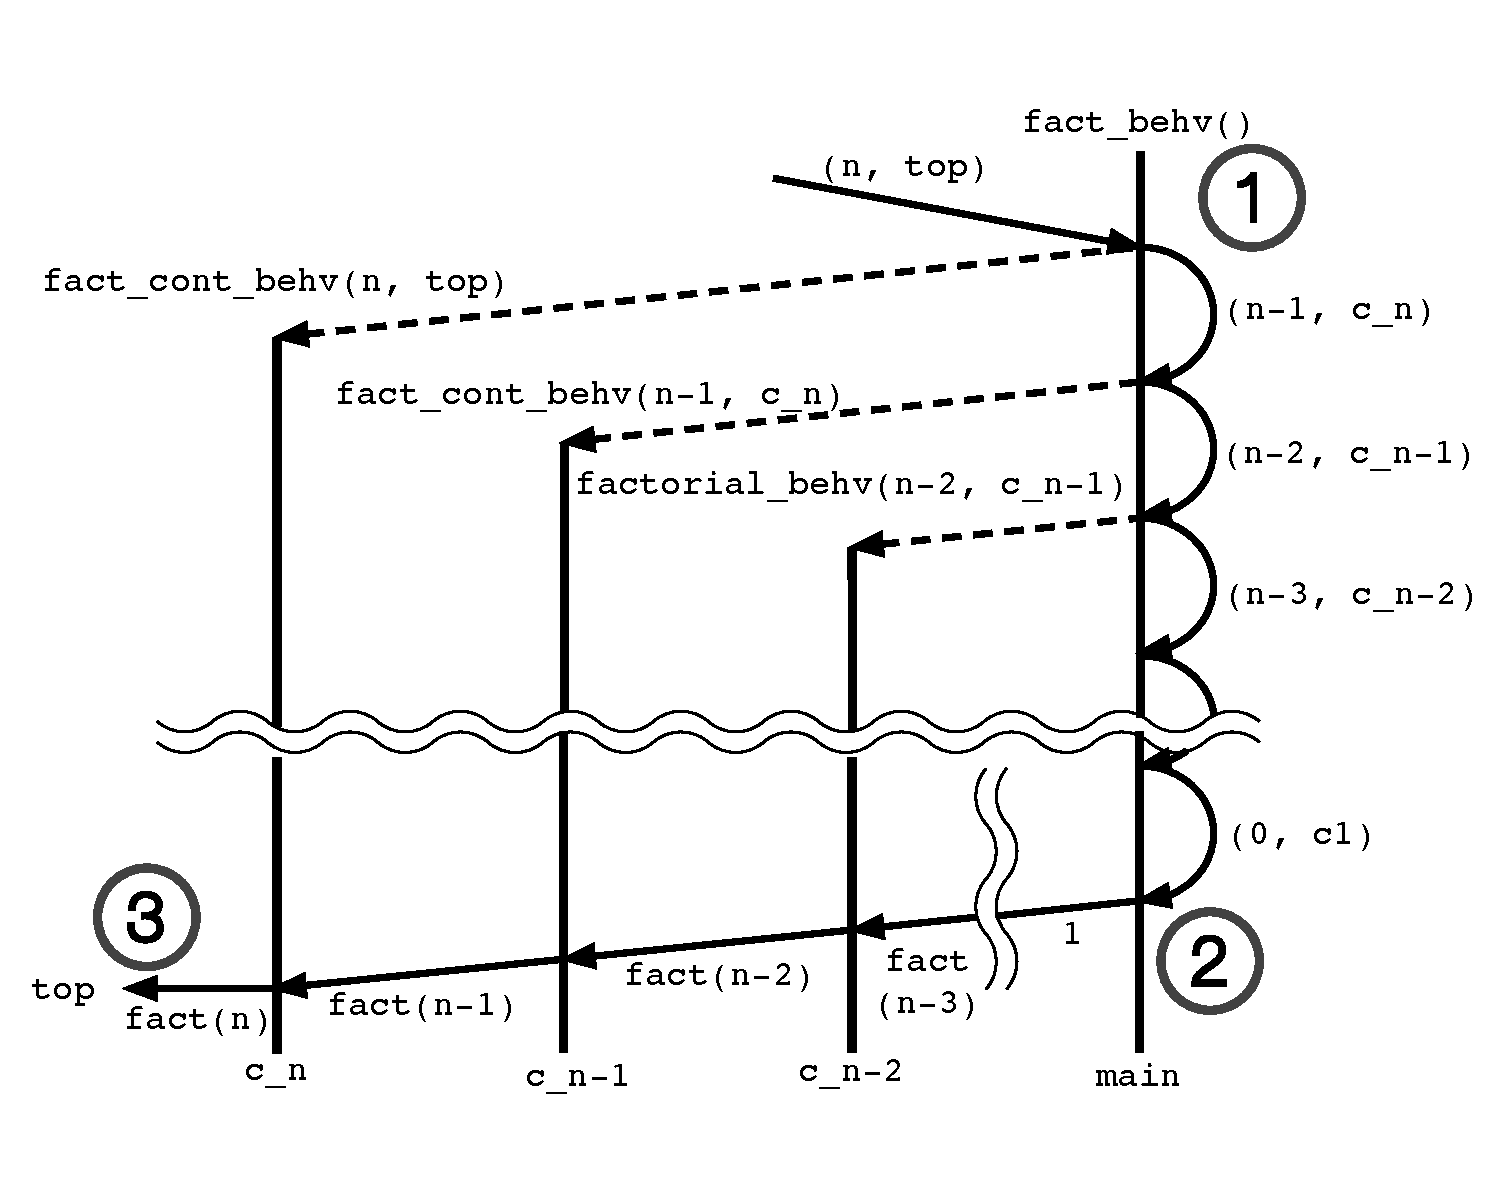
\includegraphics[width=16cm]{./img/conclusion/fact_n.pdf}
  \caption{$n$の階乗を計算するシステムの動き}\label{img:conclusion:fact}
\end{figure}

しかし,現在の証明機構では,ラベルおよびそのラベルによって遷移した後の配置を計算するために,配置内のすべてのアクターが具体的に定まっている必要がある.
このシステムでは配置内のアクターは自然数$n$によって決定するので,配置は具体的には定まらない.

また,配置を具体的に決定できなくても図\ref{code:conclusion:possible-labels-cat}の補題が成り立てば少し証明がやりやすくなるが,これは\textsc{Send}遷移の際に送り先の状態(メッセージキュー)を操作する必要があるため成り立たない.
\textsc{Send}遷移をする際に送り先のメッセージキューに直接メッセージ入れず,バッファとなるようなものを用意して一時的にその部分に保存するようにすれば,この問題は解決できるが,そのような実装にしたことで確かに具体的な配置がわからなくても証明ができるようになるか,また他の定理や証明機構に影響を及ぼさないかどうかは検証の余地がある.


\begin{figure}[tp]
\begin{lstlisting}
Lemma possible_labels_cat :
  forall c c',
    possible_labels (c ++ c') =
    possible_labels c ++ possible_labels c'
\end{lstlisting}
\caption{\coqi{possible_labels}についての補題}\label{code:conclusion:possible-labels-cat}
\end{figure}


さらに,\fairness を用いなければ証明できないような命題の証明を行えるような仕組みを整えなければいけない.
例えば,図\ref{code:conclusion:pingpong}のような,1. pingというメッセージを受け取ると,pingメッセージの送り主に対してpongというメッセージを送信するサーバ,2. サーバに対してpingというメッセージを送り続ける2つのクライアント,を考える.このシステムは図\ref{code:conclusion:pingpong-spec},つまりを満たすべきだが,
\ref{chapter:proof}で定義した\coqi{fairness}を使うためには,あるラベルが遷移可能になることが無限に繰り返されるようなパスであることを示す必要があり現状の証明機構では使いづらい.そのため,\coqi{fairness}を使いやすいようなタクティクなどの仕組みを作るか,\coqi{fairness}自体を同等または弱い性質でかつ扱いやすいものに定義し直す必要がある.

\begin{figure}[tp]
\begin{lstlisting}
(**
 * ping というメッセージを受け取ると,
 * pong というメッセージを送り主に送信する
 *)
Definition server_behavior (state : unit) : behavior unit :=
  receive (fun msg =>
         match msg with
           | tuple_msg (name_msg sender) (str_msg "ping") =>
             sender ! (str_msg "pong");
             become state
           | _ => become state
         end).

(* メッセージを受け取るとサーバに ping というメッセージを送る *)
Definition client_behavior (server_addr : name) : behavior name :=
  receive (fun _ =>
    me <- self;
    server_addr ! (tuple_msg (name_msg me) (str_msg "ping"));
    become server_addr
  ).

Definition pingpong_system : config :=
  init "pingpong" (
    server <- new server_behavior with tt; (* サーバーを作る *)
    (* クライアント1を作る *)
    client1 <- new client_behavior with server;
    (* クライアント2を作る *)
    client2 <- new client_behavior with server;
    client1 ! empty_msg; (* クライアント1を走らせる *)
    client2 ! empty_msg; (* クライアント1を走らせる *)
    become done (* それ以降は何もしない *)
  ).
\end{lstlisting}
  \caption{ping-pongシステム}\label{code:conclusion:pingpong}
\end{figure}

\begin{figure}[tp]
\begin{lstlisting}
Definition client1_name := generated 1 (toplevel "pingpong").
Theorem receive_client1 :
  eventually_receive pingpong_system
    (generated 1 top) (str_msg "pong").
\end{lstlisting}
  \caption{ping-pongシステムが満たすべき性質}\label{code:conclusion:pingpong-spec}
\end{figure}

\subsection{障害の形式化}
本ライブラリの最終目標としては,障害が起こりうる環境においてもシステムの性質は成り立つというような命題に対して検証を行えるというものだったが,それはまだ達成できていない.
これを達成するためには,まず障害を形式化し障害を含むような意味論にすること,障害から復旧させるような機構を導入すること,が挙げられる.

%% 障害を含むような意味論は図\ref{code:conclusion:failure}のようなものになると考えられる.

%% \begin{figure}
%% \label{code:conclusion:failure}
%% \caption{障害を含むような意味論}
%% \end{figure}

また,障害を含むような場合と障害を含まないような場合で分けて検証できるように,意味論を切り替えられるようにすることが必要である.
この手法はVerdiが行っているもので,こうすることによって,ある障害については耐性があるが,別のある障害に対しては耐性がない,というようなことも検証できるようになる.


\section{まとめ}

本論文では,アクターシステムの検証ライブラリActarioを提案した.
ActarioはまずActarioが提供する構文を用いてアクターシステムを記述し,その性質をActarioの補題とタクティクを使って検証,そしてErlangに抽出するというものである.これらを実例を見ながら説明した.
Actarioではアクターの名前はシステムによって暗黙的につけられるようになっており,またその名前付けの一意性はCoqにより形式的に証明されている.
アクターシステムの検証を簡単にするための機構,そして抽出の方法について説明した.

Actarioを使って検証したアクターシステムの例は簡単なものだけであり,またアクターシステムの検証のための補題やタクティクも少ないので,まだまだ実用的ではないと言わざるを得ない.
大規模で複雑なシステムの検証のため補題やタクティクを補強することが課題である.


\chapter*{謝辞}
\addchapter{謝辞}
本研究を行うにあたり,ご指導いただきました渡部卓雄准教授に深く感謝致します.
また,様々な助言をくださった渡部研究室の皆様に感謝致します.
%% 渡部研究室の同期に感謝致します.を入れたいが,

\bibliographystyle{jplain}
\bibliography{./references}

\appendix
\chapter{ラベル付き遷移システムのCoqによる形式化}
\label{appendix:trans}
\lstinputlisting[style=small]{./code/appendix/trans.v}

\chapter{遷移後の配置を計算する関数}
\label{appendix:calc-trans}
\lstinputlisting[style=small]{./code/appendix/calc-trans.v}


\end{document}
